\capitulo{6}{Trabajos relacionados}

Vamos a hacer un pequeño resumen de las mejores herramientas ya existentes que realizan algo muy similar al proyecto aquí expuesto.

\section{Cronología en Google Maps}
Sin duda para mí, la cronología de Google \cite{cronologia} es la reina indiscutible en este apartado. Se trata de un recolector profesional de ubicaciones, que incluso pausándolo, recolecta tu posición si por ejemplo tienes activado la \textit{Actividad en la Web y en Aplicaciones} (algo que viene por defecto) para personalizar los resultados de tu búsqueda, en función de tu posición o si haces una foto, para añadir la posición donde fue tomada.
Además añade en tu ruta establecimientos visitados, tiempo de visita y no tiene miedo a pronosticar dónde vives o dónde está tu trabajo, gracias a sus algoritmos.

Cuenta con una interfaz muy simple, accesible tanto desde el ordenador como a través de la aplicación móvil de Google Maps, que te permite ver tu recorrido a lo largo de un día cualquiera, gracias a la antena GPS que incorpora tu dispositivo.
Con unos conocimientos avanzados sí se podría desactivar por completo, se puede editar alguna entrada específica o incluso borrarla y por supuesto, es privada.
Descompresión del \textit{zip} generado por MyGeodata.
\begin{figure}[!h]
	\centering
	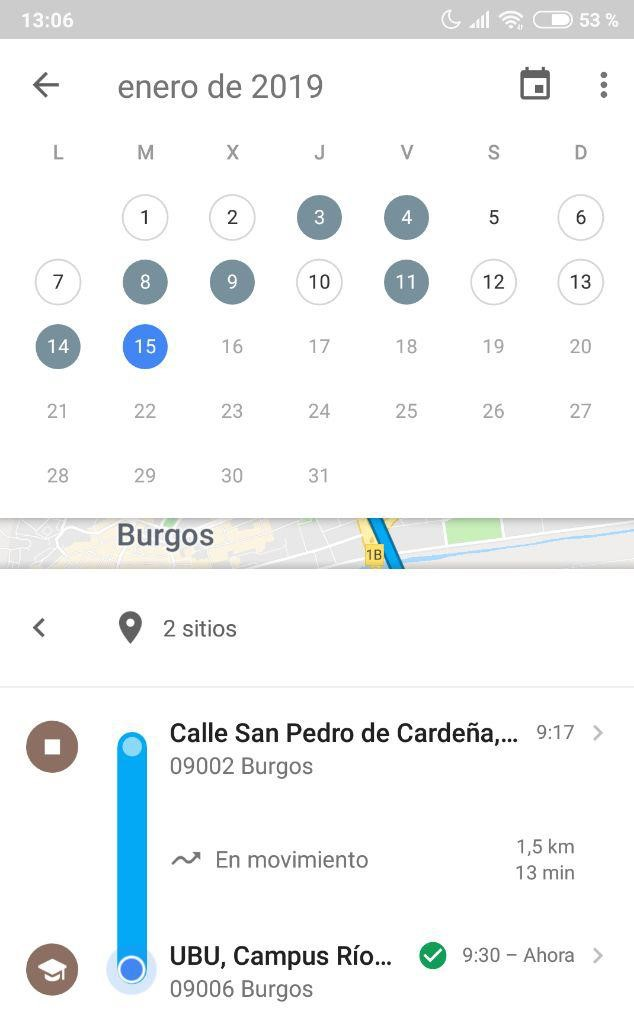
\includegraphics[width=0.4\textwidth]{cronologia.PNG}
	\caption{Se muestran todos los trayectos que se realicen en el día.}\label{fig:cronologia.PNG}
\end{figure}
\FloatBarrier
\begin{figure}[!h]
	\centering
	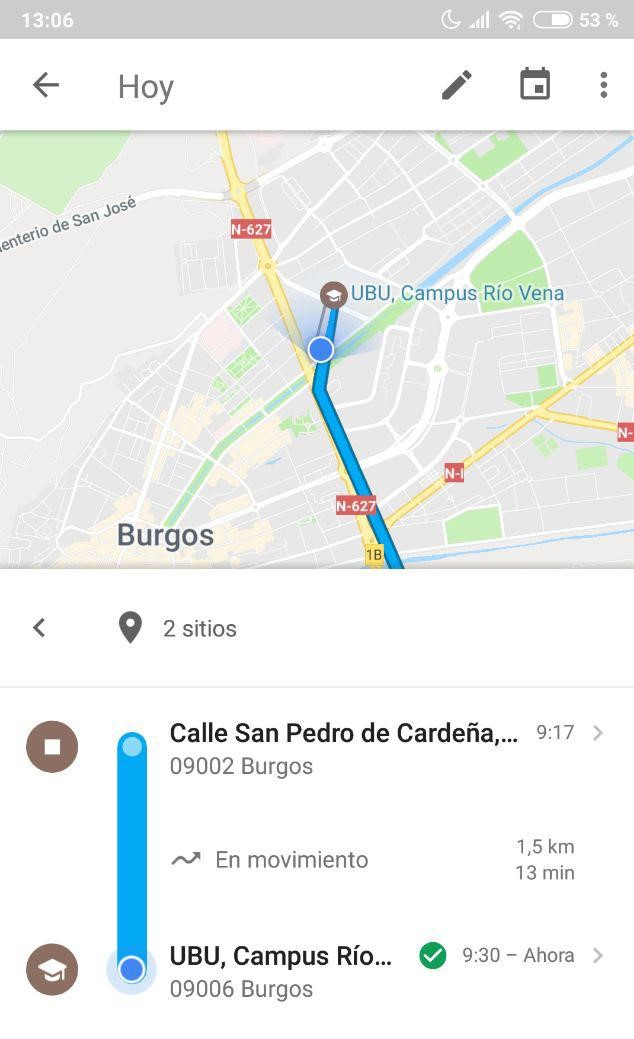
\includegraphics[width=0.4\textwidth]{cronologia2.PNG}
	\caption{Se puede seleccionar cualquier día, desde que tenga datos.}\label{fig:cronologia2.PNG}
\end{figure}
\FloatBarrier

\section{Endomondo}
Endomondo \cite{endomondo} es una aplicación móvil diseñada especificamente para deportistas. Si bien, aparte de recoger la ruta aporta otras muchas opciones y características, realiza la captura de datos de forma correcta gracias al GPS integrado del móvil, pero a diferencia de la anterior, en este caso, tú marcas cuando empieza a registrar tu ruta. Al final de la misma te dice kilómetros recorridos, tiempo invertido, velocidad media, etc.

Cuenta con la posibilidad de crear grupos entre amigos para poder retarles en una misma ruta y así poder comparar tiempos de forma directa a través de la aplicación.
Destaca su amplia compatibilidad con otros dispositivos y cuentas (Garmin Connect, Polar Flow, TomTom MySports o Fitbit) para sumar funcionalidades a la aplicación.

\section{Strava}
Otra aplicación diseñada directamente para el público más deportista, Strava \cite{strava} es considerada la red social de los \textit{runners}, altamente compatible con los pulsómetros más avanzados del mercado, permite una alta interacción entre los usuarios pudiendo ver las rutas de otros y sus estadísticas.

\section{Relive}
La última a comparar Relive \cite{relive}, a pesar de recoger la ruta como los dos anteriores, de forma tradicional y manual, cuenta con algo diferencial, y es la forma en la que es capaz de representar los mapas. Se muestran en forma de vídeo 3D, recreando la ruta por donde has ido pasando e incluyendo fotos y vídeos que hayas hecho por el camino si así lo deseas.
\begin{figure}[!h]
	\centering
	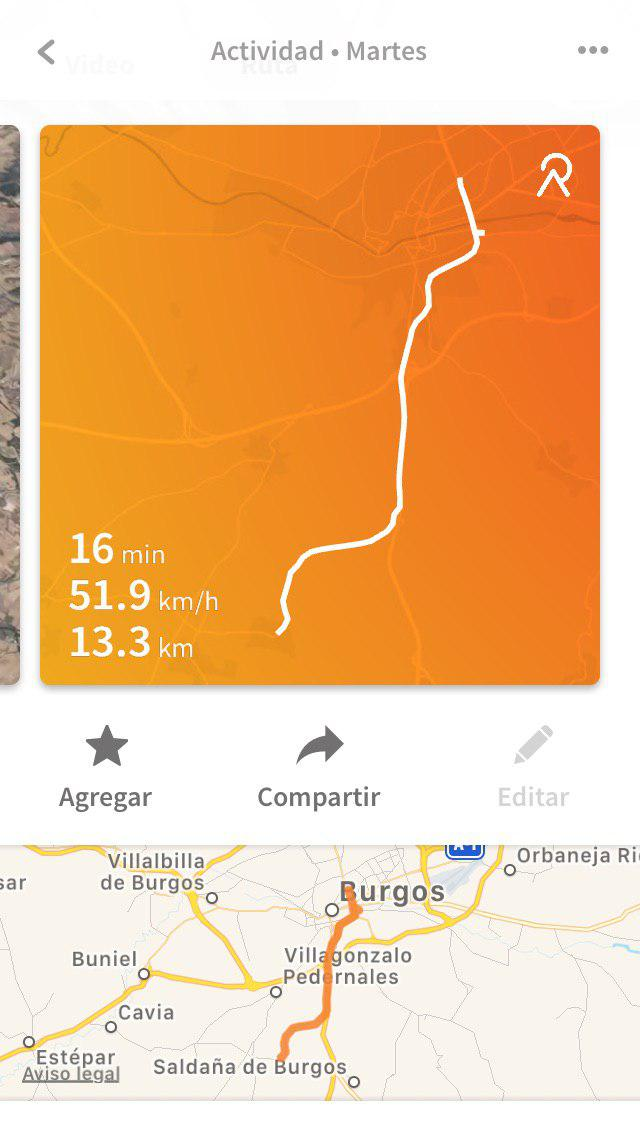
\includegraphics[width=0.4\textwidth]{relive.PNG}
	\caption{Ruta completa tradicional realizada en 2D.}\label{fig:relive.PNG}
\end{figure}
\FloatBarrier
\imagen{relive2.PNG}{Vídeo en 3D recorriendo todos los puntos por los que se ha pasado.}

\section{Conclusión}
Como comentario adicional a todas estas aplicaciones móviles cabe destacar que en mi caso no dispongo de un smartphone, se trata de un registrador de bajo costo, no asociado a ningún terminal móvil y que además almacena las posiciones en una tarjeta microSD. Las aplicaciones finales de este dispositivo podrían ser otras muy diferentes como poder acoplarlo en un coche o en una bici y tener un registro de rutas.


